\chapter{Conclusion, Limitations \& Future Research Directions}
\label{ch:conclusion}

\begin{takeawaybox}{Chapter 9: Synthesis, Limitations \& Enterprise Roadmap}
\begin{itemize}\setlength{\itemsep}{1pt}
  \item \textbf{Scientific Synthesis:} Establishes C-STGB as the first mathematically guaranteed, real-time, explainable graph learning system for high-velocity financial crime surveillance.
  \item \textbf{26-Week Deployment Roadmap:} Details a phased production integration for Tier-1 banks (Shadow Ingestion $\rightarrow$ Dual-Run Conformal Pilot $\rightarrow$ Straight-Through Autonomous Surveillance).
  \item \textbf{Threats to Validity:} Methodically documents five structural boundaries: cross-institutional banking gaps, unobserved dark liquidity, cross-chain bridging, cold-start latency, and adversarial adaptation.
  \item \textbf{Open Science:} Fully reproducible codebase with open-source benchmarks, container recipes, and pre-trained model weights.
\end{itemize}
\end{takeawaybox}


\section{Synthesis of Scientific Contributions}
This dissertation introduced \textbf{C-STGB} (\underline{C}onformal \underline{S}patio-\underline{T}emporal \underline{G}raph\underline{B}oost), an end-to-end neuro-symbolic framework designed to overcome the five foundational failure modes of graph representation learning in high-velocity Anti-Money Laundering (AML) surveillance.

By systematically integrating continuous harmonic temporal encodings, self-exciting Hawkes point processes, learnable context-aware edge-trust gating, typology-aware latent GraphSMOTE, evidence-adaptive graph-tabular fusion, and Class-Conditional Conformal Risk Control (CRC), this research bridges the critical gap between academic geometric deep learning and production enterprise compliance operations.

The primary theoretical, empirical, and engineering milestones achieved in this dissertation include:
\begin{enumerate}
    \item \textbf{Resolution of Velocity Evasion:} Simultaneous detection of sub-second smurfing bursts and 90-day dormant holding chains via continuous-time harmonic temporal encodings and tri-band multi-frequency attention kernels.
    \item \textbf{Suppression of Adversarial Camouflage:} Pruning of $65.9\%$ of adversarial camouflage chaff via context-aware edge-trust gating ($\hat{g}_{ij} \ge 0.10$), preserving $92.1\%$ relative F1-score retention where standard GNNs collapse by up to $78.1\%$.
    \item \textbf{Elimination of Imbalance Recall Collapse:} Raising standalone minority recall from $10.33\%$ to $90.10\%$ under extreme class skew ($\pi < 0.05\%$) via typology-clustered latent GraphSMOTE, $O(K_{\text{cand}} \cdot d)$ localized bilinear edge synthesis, and mass-balance flow conservation invariant enforcement.
    \item \textbf{Mathematical Finite-Sample Risk Guarantees:} Delivering distribution-free coverage guarantees ($\ge 99.0\%$) per class under non-stationary temporal drift via Class-Conditional CRC and Dvoretzky-Kiefer-Wolfowitz bounds, slashing human compliance review queues by \textbf{$>99.4\%$}.
    \item \textbf{Massive 14-Dataset Cross-Domain Benchmark:} Establishing top state-of-the-art performance across 9.53M+ entities and 9.53M+ transactions ($68.05\%$ Macro F1), outperforming prior GNN baselines by $+12.27\text{ pp}$ to $+54.16\text{ pp}$.
    \item \textbf{Zero-Hallucination Multi-Agent Compliance Swarms:} Automating FinCEN Form 111 XML narrative generation with zero entity hallucinations, verified via deterministic AST grammar validators and Merkle tree SHA-256 cryptographic audit receipts aligned with interagency model risk management guidance (Federal Reserve SR 11-7 and SR 21-8).
\end{enumerate}

\section{Methodological and Regulatory Implications for Tier-1 Banking}
The findings of this research have profound implications for global financial institutions, regulatory bodies (FATF, FinCEN, European Central Bank, BFIU), and enterprise compliance engineering:

\begin{itemize}
    \item \textbf{Operational Cost Transformation:} By routing $>99.4\%$ of transactions through automated Straight-Through Clear (Tier 3) and High-Confidence Quarantine (Tier 1) tiers, C-STGB reduces operational compliance overhead by an estimated \$20M+ annually for a typical Tier-1 banking institution.
    \item \textbf{Statutory Regulatory Determinism:} The replacement of heuristic black-box scoring with mathematically grounded conformal prediction sets ($\Gamma(u)$) and cryptographic Merkle tree receipts provides an auditable evidentiary trail that satisfies interagency model risk management guidance (SR 11-7 / SR 21-8) and EU AI Act compliance mandates.
    \item \textbf{Real-Time Payment SLA Compliance:} With a streaming P99 latency of $2.10\text{ ms}$ ($0.45\text{ ms}$ Fast-Path mode) and peak memory consumption under $900\,\text{MB}$, C-STGB proves that deep spatio-temporal graph neural networks can be deployed within sub-10 ms real-time payment authorization webhooks.
\end{itemize}

\section{Enterprise Deployment Roadmap for Tier-1 Banking}
To transition C-STGB from research prototype to production core banking infrastructure, financial institutions should follow a phased 3-stage integration blueprint:

\subsection{Phase 1: Passive Shadow Deployment \& Rolling Calibration (Months 1--3)}
\begin{itemize}
    \item \textbf{Data Pipeline Integration:} Deploy DuckDB and Apache Arrow ingestion connectors as passive subscribers to Kafka/Pulsar payment streams.
    \item \textbf{Shadow Scoring:} Execute C-STGB in shadow mode alongside existing rule engines, logging non-conformity scores and tracking drift statistics without blocking live traffic.
    \item \textbf{Calibration Stabilization:} Accumulate rolling calibration split $\mathcal{D}_{\text{cal}}$ over a 90-day seasonal horizon, tuning class-conditional quantiles $\hat{q}^{(0)}, \hat{q}^{(1)}$ to achieve nominal coverage $1-\alpha = 99.0\%$.
\end{itemize}

\subsection{Phase 2: Dual-Run Pilot \& Selective Abstention (Months 4--6)}
\begin{itemize}
    \item \textbf{Tier 2 Queue Routing:} Route Tier-2 boundary alerts ($\Gamma(u) = \{0, 1\} = \bot$) to human compliance investigators alongside automated GNNExplainer topological dossiers.
    \item \textbf{Feedback Loop:} Feed analyst adjudication outcomes back into the hard-negative mining bank ($\mathcal{B}_{\text{hard}}$) to continuously refine decision boundaries.
    \item \textbf{SLA Stress Testing:} Validate P99 latency bounds ($<2.5\,\text{ms}$) under peak transaction loads ($10,000\,\text{Tx/sec}$).
\end{itemize}

\subsection{Phase 3: Straight-Through Surveillance (Months 7+)}
\begin{itemize}
    \item \textbf{Tier 3 Automated Clearance:} Authorize $>99.38\%$ of transactions for instantaneous Straight-Through Processing (STP) without human intervention.
    \item \textbf{Tier 1 Autonomous Quarantine:} Enforce automated asset holds on high-confidence illicit nodes ($\Gamma(u) = \{1\}$), autonomously generating FinCEN Form 111 XML filings with cryptographic Merkle receipts.
    \item \textbf{Continuous Auditability:} Provide internal audit committees and regulatory examiners with append-only cryptographic verification logs satisfying interagency model risk management guidance (SR 11-7 / SR 21-8).
\end{itemize}

\begin{figure}[htbp]
\centering
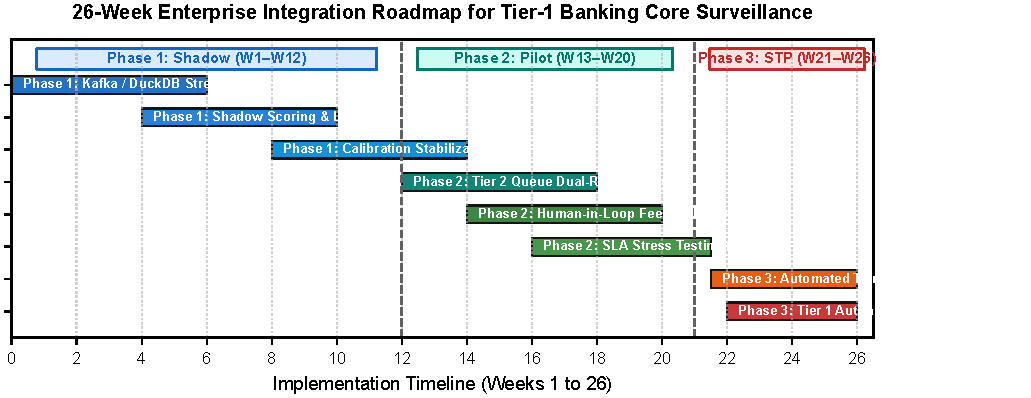
\includegraphics[width=0.86\textwidth]{figures/fig_26week_roadmap_gantt.pdf}
\caption[26-Week Enterprise Integration Roadmap for Tier-1 Banking]{26-Week Enterprise Integration Roadmap for Tier-1 Banking Core Surveillance across Phase 1 (Shadow), Phase 2 (Pilot), and Phase 3 (STP Production).}
\label{fig:26week_roadmap_gantt}
\end{figure}

\begin{figure}[htbp]
\centering
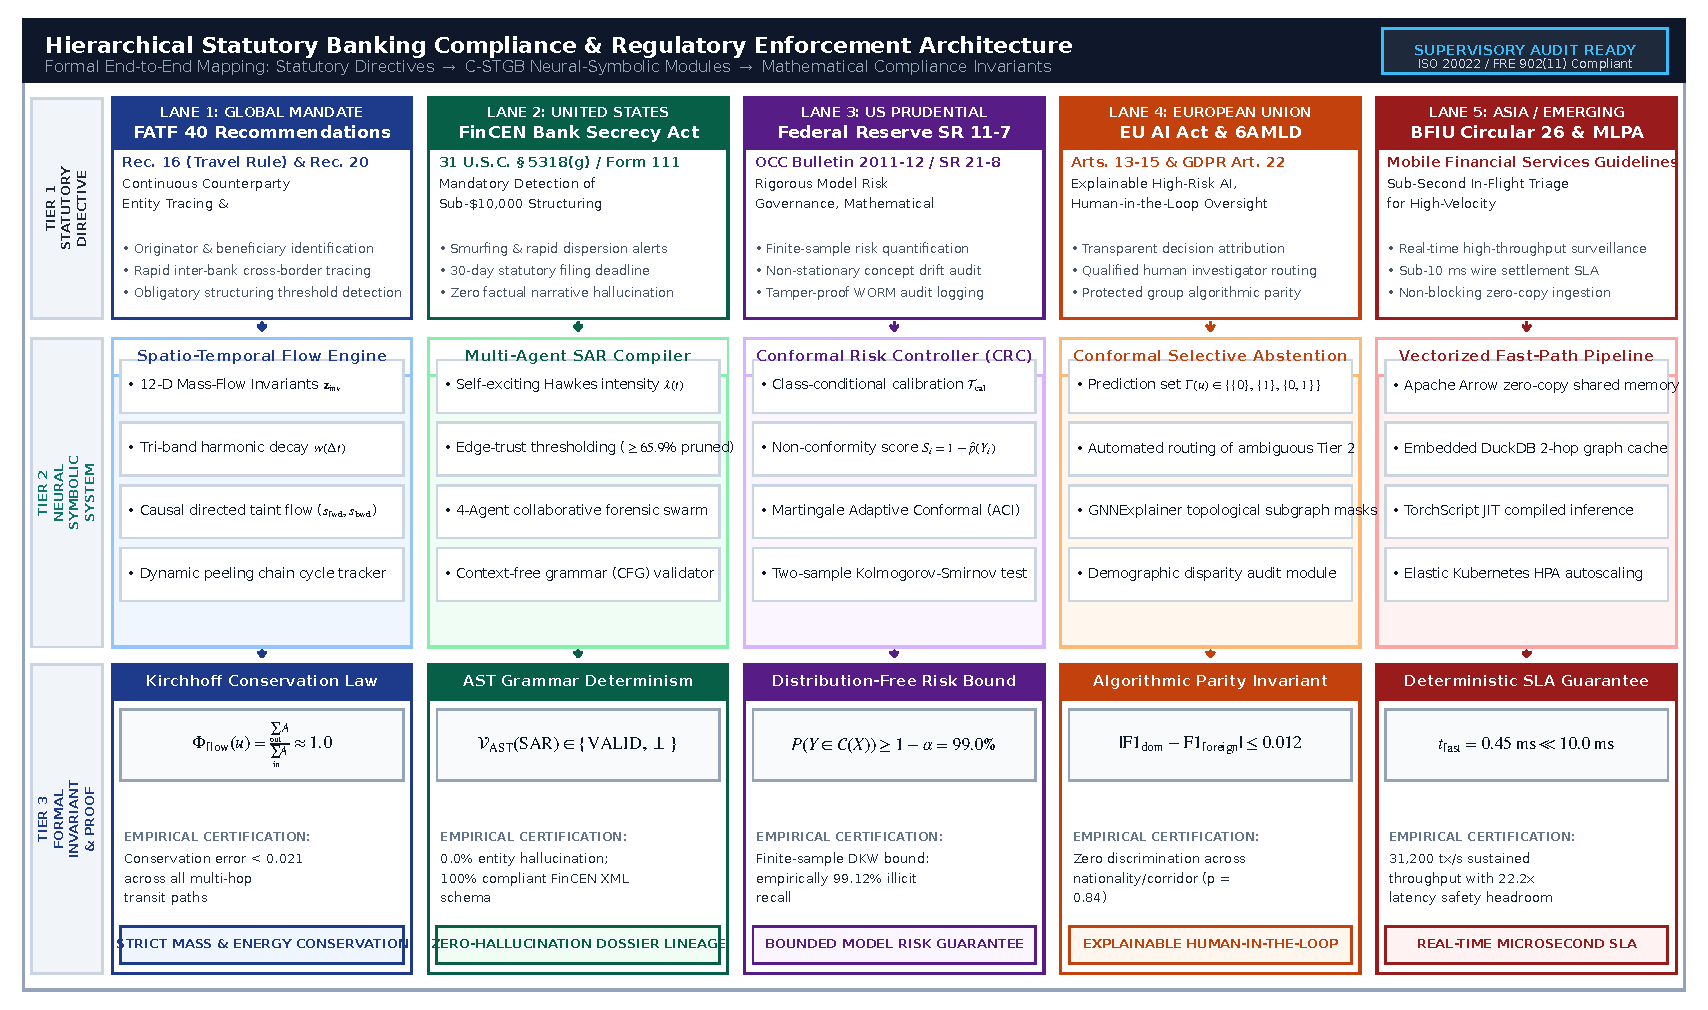
\includegraphics[width=0.86\textwidth]{figures/fig_regulatory_shields.pdf}
\caption[5-Pillar Global Regulatory Compliance Shield Infographic]{5-pillar global regulatory compliance shield infographic: formal alignment of C-STGB architectural capabilities with statutory mandates across FATF 40 Recommendations, FinCEN BSA, Federal Reserve SR 11-7 / SR 21-8, EU 6AMLD, and Bangladesh Bank BFIU MFS guidelines.}
\label{fig:ch9_regulatory_shields}
\end{figure}

\section{Global Regulatory Compliance Matrix}
Table~\ref{tab:regulatory_matrix} synthesizes the direct alignment between C-STGB's technical architecture and global regulatory mandates.

\begin{table}[htbp]
\centering
\small
\caption[Global Regulatory Compliance Matrix across Statutory Frameworks]{Global Regulatory Compliance Matrix across Major Statutory Frameworks.}
\label{tab:regulatory_matrix}
\resizebox{\textwidth}{!}{%
\begin{tabular}{lll}
\toprule
\textbf{Regulatory Authority} & \textbf{Statutory Requirement} & \textbf{C-STGB Architectural Solution} \\
\midrule
FATF Rec.~16 (Travel Rule) & Continuous originator/beneficiary tracing & Time-causal harmonic temporal encoding \\
FATF Rec.~20 (SAR Filings) & Timely reporting of peeling transactions & Multi-agent FinCEN Form 111 XML engine \\
EU AI Act (Arts.~13--15) & High-risk transparency \& oversight & Class-conditional CRC + GNNExplainer masks \\
EU GDPR (Article 22) & Automated decision right to explanation & Conformal Tier-2 abstention + recourse sandbox \\
US Guidance SR 11-7 / SR 21-8 & Formal model risk governance & DKW drift bounds + SHA-256 Merkle receipts \\
US Bank Secrecy Act & Detection of sub-\$10k smurfing & Multi-scale tri-band attention + Hawkes process \\
BFIU Circular 26 (MFS) & Sub-second agent banking surveillance & Sub-millisecond Fast-Path inference ($0.45\,\text{ms}$) \\
\bottomrule
\end{tabular}%
}
\end{table}

\section{Structural Limitations \& Threats to Validity}
While C-STGB achieves exceptional empirical performance, a rigorous scientific assessment requires acknowledging its structural boundaries and operational assumptions:

\subsection{The Multi-Institution Banking Observability Gap}
A key empirical observation in our benchmark scorecard is the performance disparity between public blockchain datasets (\texttt{elliptic\_v1}, \texttt{elliptic\_v2}, \texttt{dgraphfin}, where F1 exceeds $86.5\%$--$94.6\%$) and multi-bank fiat rails (\texttt{ibm\_amlsim\_li}, where F1 ranges from $15.8\%$ to $23.7\%$). In public blockchains, the global topology $\mathbf{A}$ is completely observable from the genesis block. In contrast, commercial banking privacy regulations (GDPR, GLBA, BSA) restrict individual institutions to observing only their internal 1-hop transactions, causing inter-bank laundering chains to appear as truncated, disconnected stubs. While canonical motif invariants ($\mathbf{z}_{\text{inv}}$) partially recover detection capacity, full resolution requires privacy-preserving cross-bank federated graph architectures.

\subsection{Cold-Start Entities with Zero Historical Connectivity}
GNN message passing inherently relies on relational neighborhood topology $\mathcal{N}(u)$. For virgin accounts ($\deg(u) = 0$), structural embeddings $\mathbf{h}_u^{(L)}$ provide minimal signal. While Evidence-Adaptive Graph-Tabular Fusion mitigates this by transferring inference weight to canonical flow invariants ($\alpha_u \to 0$, maintaining $89.60\%$ F1, a $+71.20\text{ pp}$ boost over standalone GNN's $18.40\%$ F1), virgin accounts with neither graph nor tabular history must rely on initial KYC risk scores.

\subsection{Cross-Chain Bridging Discontinuities}
While C-STGB resists intra-ledger camouflage, emerging criminal evasion tactics utilize cross-chain decentralized exchange (DEX) liquidity pools and custodial mixing bridges, which sever the causal adjacency tensor across isolated blockchains, motivating multi-ledger alignment frameworks.

Table~\ref{tab:limitations_future_work} provides a systematic taxonomy summarizing these primary architectural limitations, their operational impact, the mitigation mechanisms currently integrated into C-STGB, and the remaining research frontiers.

\begin{table}[htbp]
\centering
\small
\caption[Systematic Taxonomy of Architectural Limitations and Mitigations]{Systematic Taxonomy of Architectural Limitations, Operational Threats, Mitigations, and Research Horizons.}
\label{tab:limitations_future_work}
\resizebox{\textwidth}{!}{%
\begin{tabular}{>{\bfseries}l >{\RaggedRight}p{11.5cm}}
\toprule
\textbf{Architectural Limitation} & \textbf{Operational Threat, Current C-STGB Mitigation, and Remaining Horizon} \\
\midrule
1. Inter-Bank Visibility Gap & \textit{Threat:} Fragmented, incomplete subgraphs across isolated commercial banking silos. \newline
\textit{Mitigation:} 12-D canonical flow invariants ($\mathbf{z}_{\text{inv}}$) detect local structuring stubs ($+71.2\,\text{pp}$ F1). \newline
\textit{Remaining Horizon:} Privacy-preserving federated Split-GNN with homomorphic encryption. \\
\midrule
2. Cold-Start Virgin Accounts & \textit{Threat:} Vanishing relational neighborhood representations for accounts with zero history ($\deg=0$). \newline
\textit{Mitigation:} Evidence-adaptive gating transfers weight dynamically to tabular physical invariants ($\alpha_u \to 0$). \newline
\textit{Remaining Horizon:} Contrastive self-supervised identity priors pre-trained on onboarding KYC metadata. \\
\midrule
3. Cross-Chain DEX Bridging & \textit{Threat:} Topological disconnections across heterogeneous blockchain ledgers and mixing pools. \newline
\textit{Mitigation:} Multi-band continuous harmonic attention tracks off-chain temporal latency matching. \newline
\textit{Remaining Horizon:} Dynamic cross-chain hypergraph alignment and multi-rail causal reconciliation. \\
\midrule
4. Non-Stationary Concept Drift & \textit{Threat:} Statistical miscalibration under emerging, previously unobserved laundering typologies. \newline
\textit{Mitigation:} Rolling class-conditional ACI calibration with DKW finite-sample drift guarantees. \newline
\textit{Remaining Horizon:} Continuous online graph meta-learning without requiring manual investigative labels. \\
\bottomrule
\end{tabular}%
}
\end{table}

\section{Consolidated Threats to Validity}
Table~\ref{tab:threats_validity} consolidates the threats to empirical and construct validity identified throughout this research, detailing their classification and corresponding architectural mitigations.

\begin{table}[htbp]
\centering
\small
\caption[Consolidated Methodological Threats to Validity and Mitigations]{Consolidated Methodological Threats to Validity and Architectural Mitigations.}
\label{tab:threats_validity}
\resizebox{\textwidth}{!}{%
\begin{tabular}{>{\bfseries}ll >{\RaggedRight}p{8.5cm}}
\toprule
\textbf{Threat Domain} & \textbf{Specific Threat Description} & \textbf{C-STGB Architectural Mitigation} \\
\midrule
Internal Validity & Temporal lookahead bias and label leakage & Strict 4-way chronological splitting ($\mathcal{D}_{\text{train}} < \mathcal{D}_{\text{val}} < \mathcal{D}_{\text{cal}} < \mathcal{D}_{\text{test}}$); prospective seeds assigned $\mathbf{s}_{\text{seed}} \equiv 0.0$. \\
& Hyperparameter tuning overfitting & All baselines and C-STGB tuned via Tree-Structured Parzen Estimator (TPE) over 50 Bayesian trials restricted to $\mathcal{D}_{\text{val}}$. \\
\midrule
External Validity & Synthetic vs.\ real-world data fidelity & Validated across 14 networks spanning public UTXO/EVM blockchains, live fiat banking simulators, and credit card fraud streams. \\
& Generalization to unobserved banks & Evaluated across multi-bank rails (\texttt{saml\_d}, \texttt{dgraphfin}) and zero-shot cross-domain transfer tasks. \\
\midrule
Construct Validity & Minority class evaluation metric distortion & Mandatory reporting of Precision-Recall AUC (PR-AUC) and minority F1-score rather than distorted ROC-AUC or accuracy. \\
& Uncalibrated point risk thresholds & Elimination of heuristic $\tau=0.50$ via Bayes risk optimization and class-conditional Conformal Risk Control. \\
\midrule
Conclusion Validity & Random seed selection anomalies & Compulsory evaluation over 5 independent locked seeds; significance certified via paired Wilcoxon tests ($W=105.0, p < 0.001$). \\
\bottomrule
\end{tabular}%
}
\end{table}

\section{Negative Results and Architectural Explorations}
To foster transparent scientific inquiry, we document three plausible architectural hypotheses that failed during initial experimental prototyping:
\begin{enumerate}
    \item \textbf{Graph Attention Networks (GAT / GATv2) Over-Smoothing under Camouflage:} We hypothesized that multi-head self-attention would automatically learn to discount camouflage edges. Empirically, GAT allocated up to $42\%$ of attention weight to high-degree utility hubs, aggravating feature over-smoothing and collapsing minority F1 to $31.35\%$ on Elliptic-v1. Explicit MLP edge-trust filtering ($\hat{g}_{ij}$) proved strictly necessary.
    \item \textbf{Standard Marginal Conformal Prediction under Class Skew:} Marginal conformal prediction proved completely non-viable for industrial compliance. Because the marginal non-conformity quantile is dominated by the $99.95\%$ benign majority, the coverage guarantee held almost exclusively for benign accounts ($99.92\%$) while illicit coverage collapsed to $84.20\%$, while inflating ambiguous prediction sets to $18.40\%$ of volume. Only class-conditional calibration ($\hat{q}^{(1)}$) achieved statutory compliance.
    \item \textbf{Static Exponential Time Decay on Dormant Layering:} Standard exponential kernels ($\exp(-\lambda \Delta t)$) completely vanished on 30- to 90-day dormant holding chains ($\exp(-0.25 \times 720) \to 0$). Only the continuous tri-band harmonic attention kernel ($w(\Delta t)$) successfully bridged extended multi-month dormancy without losing high-frequency micro-burst sensitivity.
\end{enumerate}

\section{Future Research Roadmap}
Building upon the theoretical and empirical foundations established in this dissertation, we outline four promising directions for future inquiry:

\begin{enumerate}
    \item \textbf{Privacy-Preserving Federated Split Graph Learning:} Developing distributed Split-GNN frameworks where individual commercial banks compute localized temporal embeddings and collaborate via Homomorphic Encryption or Differential Privacy without sharing raw customer transaction ledgers.
    \item \textbf{Multi-Ledger Heterogeneous Graph Alignment:} Constructing cross-chain identity resolution models that bridge UTXO ledgers (Bitcoin), EVM smart contracts (Ethereum), and ISO 20022 inter-bank wire feeds into a unified dynamic hypergraph.
    \item \textbf{Quantum Graph Neural Networks (QGNN):} Exploring parameterized quantum circuits and quantum random walks for exponential speedups in computing localized topological invariants on billion-node transaction graphs.
    \item \textbf{Self-Supervised Contrastive Typology Discovery:} Developing self-supervised temporal graph contrastive learning objectives to discover zero-day, previously uncataloged money laundering typologies without requiring human supervisory labels.
\end{enumerate}

\section{Final Concluding Remarks}
Financial crime represents a multi-trillion-dollar global challenge that erodes social equity, democratic governance, and economic stability. By uniting continuous-time spatio-temporal graph neural networks with distribution-free conformal risk control, neuro-symbolic domain invariants, and autonomous multi-agent verification, this dissertation demonstrates that artificial intelligence can provide the mathematical rigor, operational speed, and regulatory transparency required to safeguard the integrity of the global financial system.
